\documentclass[twocolumn]{article}
\usepackage{xeCJK}
\setCJKmainfont{IPA明朝}
\usepackage[a4paper, top=1in, bottom=1in, left=2cm, right=2cm]{geometry}
\usepackage[singlespacing]{setspace}
\usepackage{amsmath}
\usepackage{amssymb}
\usepackage{graphicx}
\usepackage{hyperref}
\title{水中の鉛筆が描くアストロイド:\\光と幾何学の不思議な出会い}
\author{M. Ryu \\ {\href{mailto:mingshey@hafs.hs.kr}{mingshey@hafs.hs.kr}}}
\begin{document}
	\maketitle
	\newcommand{\romana}{{a}}
	\newcommand{\romanb}{{b}}
	\newcommand{\romanA}{{A}}
	\newcommand{\romanB}{{B}}
	\newcommand{\greeka}{{\alpha}}
	\newcommand{\greekb}{{\beta}}
	\newcommand{\Aprime}{{A^{\prime}}}
	\newcommand{\Bprime}{{B^{\prime}}}
	\renewcommand{\figurename}{図}
	\section{はじめに}
	
	水に半分浸かった鉛筆が曲がって見える現象は、誰もが一度は経験したことがある光の屈折の身近な例です(図1)。しかし、鉛筆の先端が観察する角度によって異なる位置に見えるとしたら、あなたは不思議に思ったことはありませんか?
	
	\begin{figure}[ht]
		\centering
		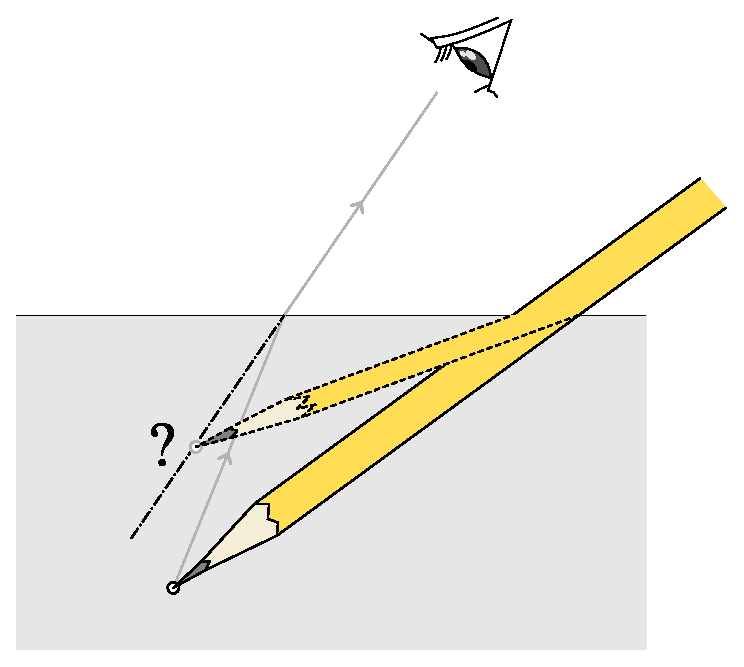
\includegraphics[width=2in]{g164.eps}
		\caption{水中の鉛筆}
		\label{fig:pencil}
	\end{figure}
	
	一般的に、物理の初歩的な学習では、真上から見たときの鉛筆の先端の位置について学ぶことが多いでしょう。しかし、斜めから見たときに鉛筆の先端がどのように見えるのかについては、詳しく説明されないことがほとんどです。より高度な光学の教科書でも、レンズや鏡といった重要な光学機器に焦点が当てられ、この現象は比較的軽視される傾向にあります。
	
	これは、この現象が比較的複雑な数学的な取り扱いを必要とするため、初学者には少し難しいという側面があること、そしてレンズや鏡のような光学機器の原理に比べると、日常的な現象としてはそれほど重要視されないという側面があるためと考えられます。
	
	しかし、このように一見単純ながらも興味深い現象は、私たちの好奇心を刺激します。筆者自身も、この現象について深く考えてみたことがあります。本稿では、この疑問に対する答えを探求し、光と幾何学が織りなす不思議な世界を覗いてみましょう。
	
	\section{まとめ:意外な答え}
	
	少し数学的な説明が続きましたが、結論を先に述べると、平らな水面の下にある物体を水面上から見ると、その像の位置は観察する角度によって変化します。そして、観察者が水面上で移動すると、その像が描く軌跡は、ある特定の数学曲線を描くことが分かりました。
	
	この軌跡は、光学で現れる「コースティック」(caustic)と呼ばれる光の集積曲線の一種で、この場合は「つぶれたアストロイド」と呼ばれる曲線になります。
	
	\begin{figure}[h]
		\centering
		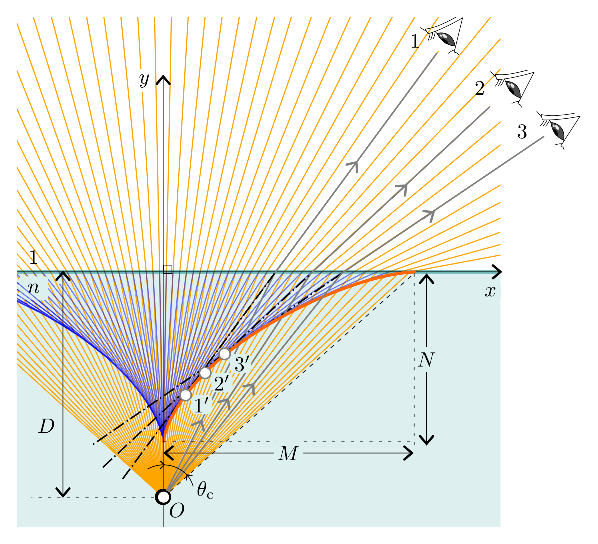
\includegraphics[width=3in]{g409.eps} \hfill\null
		\caption{観察点の位置によって変化する像の軌跡}
		\label{fig:caustic}
	\end{figure}
	
	図\ref{fig:caustic}のように、物体と観察点を結ぶ平面を考え、この平面と水面の交線を$x$軸、物体を通り水面に垂直な直線を$y$軸とします。この座標系において、像の軌跡は次のような式で表されます。
	
	$$ \left| \dfrac{x}{M} \right| ^ {2/3} 
	+ \left| \dfrac{y}{N} \right| ^ {2/3} = 1,$$
	
	ここで、$M = D/\sqrt{n^2 - 1}$は全反射の臨界角($\theta_{\mathrm{c}}$)によって決まる入射距離の最大値、$N = D/n$は真上から見たときの物体の見かけの深さ、$D$は物体の実際の深さ、$n$は空気に対する水の屈折率です。
	
	\section{光の道すじとコースティック}
	
	水中の物体から出た光は、水と空気の境界面で屈折し、私たちの目に届きます。このとき、光線の集まりが作る包絡線を「コースティック」と呼びます。コースティックは、光が集中したり、発散したりする場所を示し、私たちが物体をどのように見るかに大きく影響します。
	
	\begin{figure}[ht]
		\centering
		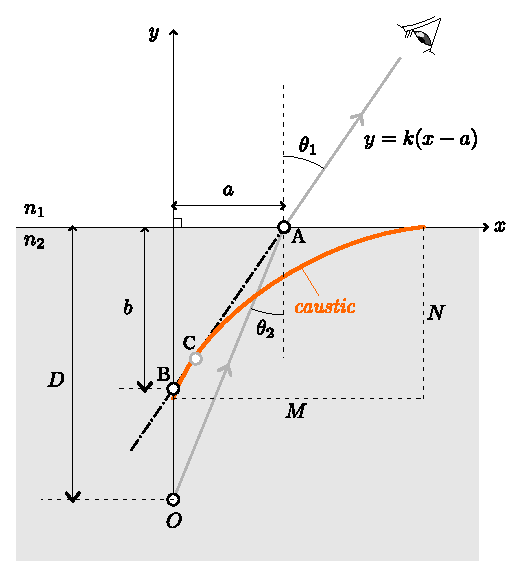
\includegraphics[width=3in]{g237.eps}
		\caption{水と空気の境界面での光の屈折とコースティック}
		\label{fig:geometry}
	\end{figure}
	
	図\ref{fig:geometry}のように、水中の点$O$から出た光が、空気との界面上の点Aで屈折し、その屈折光を逆向きに延長した直線と$y$軸との交点を${\mathrm{\romanB}}$とします。この直線${\mathrm{\romanA\romanB}}$の包絡線がコースティックとなります。
	
	スネルの法則より、入射角$\theta_2$と屈折角$\theta_1$の間には以下の関係が成り立ちます。
	$$ \sin\theta_1 = \frac{n_2}{n_1} \sin\theta_2 = n\sin\theta_2.$$
	ここで、$n$は空気に対する水の屈折率です。
	
	屈折した光線は、以下の式で表される直線上を進むと考えることができます。
	$$y=k(x-\romana).$$
	
	ここで、
	$$k=\dfrac{1}{\tan\theta_1}=\dfrac{\cos\theta_1}{\sin\theta_1}$$
	であり、スネルの法則より、
	$$k=\dfrac{\sqrt{1-n^2\sin^2\theta_2}}{n\sin\theta_2}.$$
	この直線は$y$軸と点$\mathrm{\romanB}$($y=\romanb$)で交わるため、
	$$\romanb = -k\romana.$$
	
	幾何学的な関係から、以下の式が得られます。
	$$\romana = D\tan\theta_2 = \dfrac{D\sin\theta_2}{\cos\theta_2}.$$
	したがって、
	$$\begin{aligned}
		\romanb &= -k\romana \\
		&= -\dfrac{D\sin\theta_2}{\cos\theta_2}
		\dfrac{\sqrt{1-n^2\sin^2\theta_2}}{n\sin\theta_2}\\
		&=-\dfrac{D\sqrt{1-n^2\sin^2\theta_2}}{n\cos\theta_2}.
	\end{aligned}$$
	
	ここで、無次元のパラメータ$\greeka=\romana/M$と$\greekb=\romanb/N$を導入します。
	
	$$ \begin{aligned}
		\greeka^2 + \greekb^2 &= \dfrac{\romana^2}{M^2}+\dfrac{\romanb^2}{N^2}\\
		&=\dfrac{n^2-1}{D^2}\dfrac{D^2\sin^2\theta_2}{\cos^2\theta_2}%
		+\dfrac{n^2}{D^2}\dfrac{D^2(1-n^2\sin^2\theta_2)}{n^2\cos^2\theta_2}\\
		&=\dfrac{\left(n^2-1\right)\sin^2\theta_2 + 1-n^2\sin^2\theta_2}
		{\cos^2\theta_2}\\
		&=\dfrac{1-\sin^2\theta_2}{\cos^2\theta_2}\\
		&= 1
	\end{aligned}$$
	
	ここで、無次元座標 $\xi=x/M$ と $\eta=y/N$ を導入すると、視点が$xy$平面上で移動するにつれて、点$\mathrm{A}(\romana, 0)$ と $\mathrm{B}(0, \romanb)$ もそれに応じて動き、それぞれに対応する$\xi\eta$平面上の点$\mathrm{A'}(\greeka, 0)$と$\mathrm{B'}(0, \greekb)$は、常に距離1を保ちながら動くことがわかります。
	
	このような、パラメータ$\alpha$によって表される線分$\overline{\mathrm{A'B'}}$の集合の包絡線は、「アストロイド」(図\ref{fig:astroid})と呼ばれるよく知られた曲線です。アストロイドは、次の式で表されます。
	
	$$ \left| \xi \right|^{2/3} + \left| \eta \right|^{2/3} = 1. $$
	
	つまり、水面の観察者が見ている鉛筆の先端の軌跡は、アストロイドという美しい曲線を描くのです。
	
	\begin{figure}[h]
		\centering
		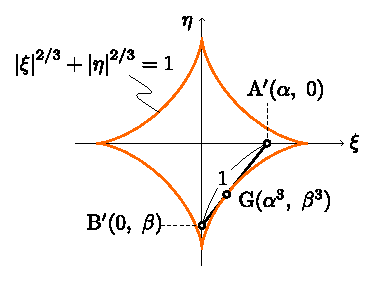
\includegraphics{g107.eps}	
		\caption{コースティックを$\xi\eta$平面に投影した図はアストロイドを描く}
		\label{fig:astroid}
	\end{figure}
	
	図\ref{fig:astroid}のように、線分$\overline{\mathrm{\Aprime\Bprime}}$とアストロイドが接する点は$\mathrm{G}(\greeka^3, \greekb^3)$であり、この点が像の位置$\mathrm{C}$に対応する。
	
	したがって、次の関係式から像の座標 $(x_{\mathrm{C}}^{}, y_{\mathrm{C}}^{})$ を得ることができます。
	$$ \left\{ 
	\begin{aligned}
		\xi_{\mathrm{G}}^{} &= \dfrac{x_{\mathrm{C}}^{}}{M} = \greeka^3 = \dfrac{\romana^3}{M^3},\\
		\eta_{\mathrm{G}}^{} &= \dfrac{y_{\mathrm{C}}^{}}{N} = \greekb^3 = \dfrac{\romanb^3}{N^3}.
	\end{aligned}
	\right.$$
	つまり、
	$$ \left\{ 
	\begin{aligned}
		x_{\mathrm{C}}^{} &= \dfrac{\romana^3}{M^2},\\
		y_{\mathrm{C}}^{} &= \dfrac{\romanb^3}{N^2}=-\dfrac{k^3\romana^3}{N^2}.
	\end{aligned}
	\right.$$
	
	ここで、
	$$\sin\theta_2 = \dfrac{\romana}{\sqrt{D^2+\romana^2}}$$
	を用いると、
	$$k = \dfrac{\sqrt{D^2-(n^2-1)\romana^2}}{n\romana},$$
	となり、像の位置を$\romana$をパラメータとする関数として表すことができます。
	$$ \left\{ 
	\begin{aligned}
		x_{\mathrm{C}}^{} &= (n^2-1)\dfrac{\romana^3}{D^2},\\
		y_{\mathrm{C}}^{} &= -\dfrac{n^2}{D^2}\dfrac{\romana^3}
		{n^3\romana^3}\left\{ D^2-(n^2-1)\romana^2 \right\}^{3/2}\\
		&=-\dfrac{D}{n}\left\{ 1-(n^2-1)\dfrac{\romana^2}{D^2} \right\}^{3/2}.
	\end{aligned}
	\right.$$
	
	\section{視点が水中にある場合}
	
	物体が高さDの空中にあり、観測者が水中にある場合、相対的な屈折率は$1/n < 1$となり、同様の推論によりコースティックに関する次の式が得られる。
	
	$$ \left| \xi \right|^{2/3} - \left| \eta \right|^{2/3} = -1, $$
	
	ここで $\xi = \dfrac{x}{W} $ および $\eta = \dfrac{y}{Z}$であり、$W = \dfrac{nD}{\sqrt{n^2-1}}$と$Z = nD$である。	
	この曲線は漸近線を持たないが、$x \to \pm\infty$のとき、傾きは$\pm Z/W = \pm \sqrt{n^2-1}$に収束する。
	
	つまり、水中から見た水面上の風景は、全反射の臨界角以内の円(あるいは円錐)内に圧縮されて見える。これは、スネルの窓と呼ばれるよく知られた現象であり、魚眼レンズのような超広角レンズで撮影された写真に見られるような、丸く広がった視野に似ている。
	
	この曲線のより一般的な形は、
	
	$$ \left| \xi \right|^{r} - \left| \eta \right|^{r} = \pm1 $$
	
	で表される曲線の族であり、\href{http://dynamicmathematicslearning.com/super-ellipse.html}{DML}\footnote{\ttfamily{dynamicmathematicslearning.com/super-ellipse.html}}では「スーパーハイパーボラ」と呼ばれ、\href{https://old.nationalcurvebank.org/superconicncb/superconicncbb.htm}{`National Curve Bank'}\footnote{\ttfamily{old.nationalcurvebank.org/superconicncb/\\superconicncb.htm}}では、アストロイドが属する
	
	$$ \left| \xi \right|^{r} + \left| \eta \right|^{r} = 1. $$
	
	のような曲線と共に「スーパーコニック」という総称で呼ばれる、広範な曲線の族の一部である。
	
	$$ \left| \xi \right|^{2/3} - \left| \eta \right|^{2/3} = \pm1 $$
	
	という特殊な場合、水上の点光源から出て水中に入射する光のコースティック曲線として物理的な意味を持ち、アストロイドとの関係が楕円に対する双曲線のような関係にあることから、「ハイパーアストロイド」と呼ぶのも興味深い。
	
	\begin{figure}
		\centering
		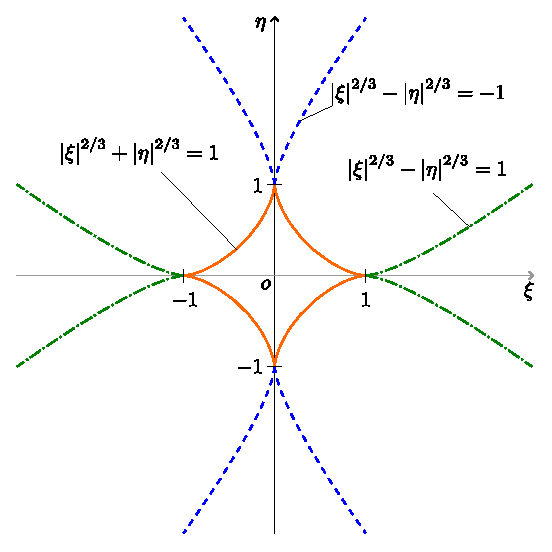
\includegraphics[width=3in]{g254.eps}
		\caption{アストロイドとハイパーアストロイド}
		\label{fig:hyperastroid}
	\end{figure}
	
	\section{像の位置を求める}
	
	物体に対する虚像のコースティックが閉じた曲線として得られたので、このコースティックを利用して、物体と視点の位置が与えられたときに、像の位置を求めることができる。
	
	\begin{figure}[ht]
		\centering
		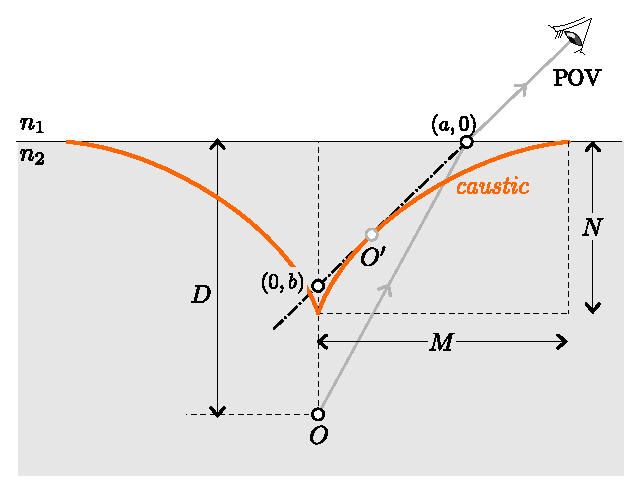
\includegraphics[width=3in]{g394.eps}
		\caption{コースティックを利用した像の位置決定}
		\label{fig:image_caustic}
	\end{figure}
	
	視点からコースティックに接線を引く。接線とコースティックの接点が像の位置であり、接線が水面と交わる点が物体から出た光線が水面に入射する点である。
	例えば、図\ref{fig:pencil_view}のように、水中に半分浸かった鉛筆の像は、観察する角度によって異なるように見える。点$1$から見ると像は$1'$の位置に、点$2$から見ると$2'$の位置に見える。
	
	\begin{figure}[ht]
		\centering
		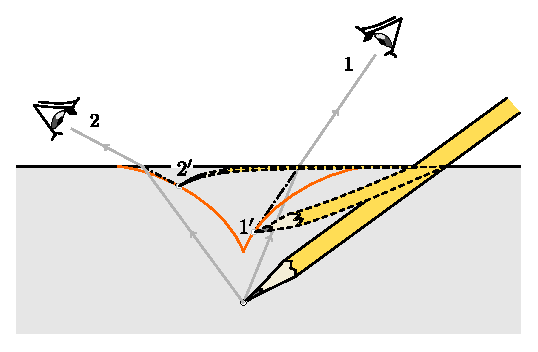
\includegraphics[width=3in]{g43.eps}
		\caption{水中に半分浸かった鉛筆の像は、観測点1, 2からそれぞれ見ると、1', 2'の位置に現れる。}
		\label{fig:pencil_view}
	\end{figure}
	
	水中に連続的な物体がある場合、物体の表面上の点$1, 2, 3, \dots$について、それぞれ上記の方法で像$1', 2', 3', \dots$を求めることができる。点が連続的に移動するとき、それに伴って移動する像の軌跡が物体の像となる。
	
	\begin{figure}[ht]
		\centering
		\includegraphics*[width=3in]{g240.eps}
		\caption{連続的な物体の像}
		\label{fig:extended_image}
	\end{figure}
	
	ただし、コースティックに対する接線を解析的に求めることは難しく、実際には数値的な方法を用いて近似的に求める必要がある。
	
	別の方法として、物体と視点とを結ぶ光線の経路をフェルマーの原理を用いて数値的に求め、光線が水面と交わる点の座標をもとに、アストロイドの接点の公式を用いて像の位置を求める方法も考えられる。この方法のPythonによる実装例は、\href{https://github.com/mingshey/python_projects/blob/main/Refraction_Image.ipynb}%
	{\sffamily{github}}\footnote{\ttfamily{https://github.com/mingshey/python\_projects/blob/main/Refraction\_Image\_en.ipynb}} で公開されている。
	
	\appendix
	\newcommand{\pd}[2]{{\frac{\partial #1}{\partial #2}}}
	\newcommand{\ilpd}[2]{{{\partial #1}/{\partial #2}}}
	\section*{付録: 包絡線としてのアストロイド}
	
	平面上の直交座標において、$x$軸上の点$(a, 0)$と$y$軸上の点$(0, b)$が常に距離$c$を維持しながら移動すると仮定しよう。このとき、$a^2+b^2=c^2$という関係が成り立ち、ある瞬間における線分を含む直線の式は以下のように表せる。
	
	$$y=-\dfrac{b}{a}(x-a)$$
	
	ここで、$b=\pm \sqrt{c^2-a^2}$を代入すると、
	
	$$y(x, a) = \mp \dfrac{\sqrt{c^2-a^2}}{a}(x-a)$$
%	
	となる。$a$の値が変化すると、2点を結ぶ線分も変化する。このような線分の集まりが作る包絡線は、$a$がわずかに変化しても変わらない点、すなわち$\ilpd{y}{a} = 0$を満たす点の軌跡として定義できる。この条件を満たす$(x, y)$を求めるために、$y$を$a$で微分すると、
	
	$$ \begin{aligned}
		\pd{y}{a} &= \pm\left[\left( \dfrac{1}{\sqrt{c^2-a^2}}+\dfrac{\sqrt{c^2-a^2}}{a^2}\right) (x-a) + \dfrac{\sqrt{c^2-a^2}}{a} \right]\\
		&= \pm \dfrac{(a^2+c^2-a^2)(x-a)+a(c^2-a^2)}{a^2\sqrt{c^2-a^2}}\\
		&= \pm \dfrac{c^2 x - a^3}{a^2 \sqrt{c^2 - a^2}}\\
		&= 0.
	\end{aligned}
	$$
	
	したがって、定点の$x$座標は$x = a^3/c^2$となり、これを$y(x, a)$に代入すると$y$座標の値は
	
	$$ \begin{aligned}
		y(x, a) &= \mp \dfrac{\sqrt{c^2-a^2}}{a}\left(\dfrac{a^3}{c^2}-a\right)\\
		& = \pm \dfrac{\left( c^2- a^2 \right)^{3/2}}{c^2}\\
		& = \dfrac{b^3}{c^2}
	\end{aligned}
	$$
%	
	となる。つまり、定点の座標$(x, y)$は次の式を満たす。
	
	$$ \left|\dfrac{x}{c}\right|^{2/3} + \left|\dfrac{y}{c}\right|^{2/3} = 1. $$
	
	これは、よく知られたアストロイドと呼ばれる曲線の方程式である。
	
	
	\section*{謝辞}
	本論文は韓国語で執筆され、翻訳にはGoogleのGemini言語モデルが活用されました。
	
%\end{japanese}
\end{document}